%=====================================================================
%  ME319: Control Systems (Autumn 2026) - Assignment 1
%  Reinventing the Steam Engine Governor
%  Compile with pdfLaTeX (IEEEtran).  Figures are produced by ../sim/vdg_main.m
%=====================================================================
\documentclass[conference]{IEEEtran}
\IEEEoverridecommandlockouts   % unlock \thanks so the repository URL is printed
\usepackage{amsmath,amssymb,graphicx,booktabs,array}
\usepackage{tikz}
\usetikzlibrary{arrows.meta,positioning,calc,decorations.pathmorphing}
\usepackage{url}
\graphicspath{{../figs/}{figs/}}

% IEEEtran's default skips around display equations and floats are generous, and
% this paper has 20 numbered display equations.  The values below stay well inside
% the class's own limits (LaTeX's \abovedisplayskip is 12pt plus 3pt minus 7pt) but
% reclaim the vertical space needed to hold the paper inside its six-page limit.
\setlength{\abovedisplayskip}{5pt plus 1pt minus 1pt}
\setlength{\belowdisplayskip}{5pt plus 1pt minus 1pt}
\setlength{\abovedisplayshortskip}{2pt plus 1pt}
\setlength{\belowdisplayshortskip}{3pt plus 1pt minus 1pt}
\setlength{\textfloatsep}{8pt plus 2pt minus 2pt}
\setlength{\floatsep}{6pt plus 2pt minus 2pt}
\setlength{\intextsep}{7pt plus 2pt minus 2pt}
\setlength{\dbltextfloatsep}{8pt plus 2pt minus 2pt}
\setlength{\dblfloatsep}{6pt plus 2pt minus 2pt}
\setlength{\abovecaptionskip}{6pt}
\setlength{\belowcaptionskip}{2pt}

\newcommand{\dg}{\ensuremath{^{\circ}}}
% \thanks is a moving argument, so the repository URL must be made robust first
\urldef{\repourl}\url{https://github.com/ZakoAtIt/me319-viscous-drag-governor}

\begin{document}

\title{A Viscous-Drag Governor: Automatic Steam-Engine Speed\\
Regulation by Fluid-Shear Sensing}

\author{
\IEEEauthorblockN{Zayan Pasha}
\IEEEauthorblockA{Department of Mechanical Engineering\\
Indian Institute of Technology Bombay\\
Mumbai, India\\
\texttt{24b2225@iitb.ac.in}}
\thanks{Source code, figures and reproduction instructions: \repourl}
}

\maketitle

\begin{abstract}
The ungoverned steam engine of the late eighteenth century loses or gains speed in
almost direct proportion to the mechanical load on its line shaft, and can therefore
overspeed to destruction or stall. Every historical solution---from Watt's flyball to
the Porter, Proell and Hartnell governors---senses speed through the centrifugal
force of rotating masses, a force proportional to $\omega^{2}$. This paper invents a
different sensing principle: a \emph{viscous-drag governor} (VDG) in which a rotor
carried by the engine shaft shears a thin oil film that drags a concentric,
spring-restrained sensing drum. The shear torque is linear in the slip speed, so the
drum deflection is linear in $\omega$ rather than quadratic and the loop gain is
independent of operating speed. The mechanism adds only an oil film, a torsion spring
and a short lever linkage---five plain turning pairs, all of them makeable in a 1780s
workshop. A first-principles nonlinear model is derived and linearised about the
normalised operating point ($\omega_0=1$, $T_{L0}=1$), giving $G_p(s)$, $G_c(s)$ and
a fourth-order characteristic polynomial. Routh--Hurwitz analysis and the Bode
margins (PM $=66.3\dg$, GM $=12.0$~dB) confirm stability with a dominant pair at
$\omega_n=3.62$~rad/s, $\zeta=0.671$. Simulated $\pm30\%$ load steps cut the
steady-state speed error from $30\%$ to $1.76\%$, with a peak deviation of $1.85\%$
and a settling time of $1.58$~s. Adding a viscous
reset dashpot drives the steady-state error to zero while retaining a $57.1\dg$
phase margin.
\end{abstract}

\begin{IEEEkeywords}
Governor, steam engine, speed regulation, viscous shear, fluid-shear sensing,
linearisation, Routh--Hurwitz, transient response, disturbance rejection.
\end{IEEEkeywords}

%=====================================================================
\section{Introduction}\label{sec:intro}
%=====================================================================
\subsection{Industrial Context and Problem Statement}
By the 1780s a single steam engine drove an entire cotton mill through a common line
shaft and belt system. Individual machines were engaged and disengaged at will, so
the mechanical load changed abruptly and unpredictably. Because the throttle was set
by hand, the engine could not hold its speed: a heavy load slowed it to a stall, and
a machine disengaged overspeeded it, risking flywheel burst and the destruction of
the shafting~\cite{dickinson}. The problem is one of \emph{disturbance rejection}:
hold the shaft speed at its nominal value under large, unmeasured steps in load
torque, using only late-eighteenth-century mechanisms.

\subsection{Design Objectives}
This work invents a new, fully automatic speed regulator and analyses it as a
linear feedback system. The objectives are: (i) a sensing principle physically
distinct from the centrifugal sensing of every historical governor; (ii) a mechanism
that could actually have been built in the 1780s; (iii) a rigorous first-principles
model, linearised about the nominal point; (iv) closed-loop stability and
transient-response analysis with standard control tools; and (v) open-loop versus
closed-loop simulation of $\pm30\%$ step loads at $\omega_0=1$, $T_{L0}=1$.

\subsection{Assumptions}
\textbf{Physical.} (1) Small-perturbation linear dynamics about the nominal
operating point are valid, as permitted by the brief. (2) Indicated torque is
proportional to throttle opening at constant cutoff. (3) The engine and flywheel
inertia is one lumped inertia $J$, and the whole resisting torque is the mill load
$T_L(\omega)$ of Eq.~\eqref{eq:TL}; its slope at the nominal point \emph{is} the
effective viscous damping $b$, which therefore does not appear separately in
Eq.~\eqref{eq:shaft}. (4) The
throttle valve is a first-order lag of time constant $\tau_v$. (5) The oil film is
laminar and isothermal---the gap Reynolds and Taylor numbers are far below the
instability thresholds, and the film dissipates only
$c_s\omega_0^{2}\approx80$~W, under $0.5\%$ of engine power---so the shear stress
obeys Newton's law of viscosity~\cite{munson} and is linear in the slip speed.
(6) Linkages are rigid, massless and backlash-free in the
nominal model; backlash and friction are treated explicitly as failure modes in
Sec.~\ref{sec:conclusions}. (9) The nominal throttle setting $x_{v0}=1$ is half
open, giving ample headroom to reach $x_v=1.28$ without striking the wide-open stop.
\textbf{Historical.} (7) No governor is assumed to exist. (8) Only 1780s materials
and processes are permitted---cast and wrought iron, brass, wood, leather and
vegetable oil; electrical, magnetic and elastomeric components are excluded by
construction, which is why the conventional eddy-current ``drag-cup'' sensor is
not used.

%=====================================================================
\section{Conceptual Design}
%=====================================================================
\subsection{The Sensing Principle}
The proposed mechanism replaces the centrifugal flyweights with a \emph{viscous
shear element}: a shallow \emph{shear rotor} keyed to the engine shaft runs inside a
concentric, sealed oil chamber (Fig.~\ref{fig:schematic}) whose wall is the
\emph{sensing drum}. The drum is not keyed to the shaft; it is free to rotate
through a small angle about the same axis, restrained by a calibrated torsion spring
anchored to the frame. (The geometry is unrelated to the eddy-current ``drag-cup''
tachometer of later centuries, where the coupling is electromagnetic rather than
viscous.)

At constant speed the rotor drags the oil, the oil drags the drum, and the drum
comes to rest at the angle at which the transmitted shear torque is exactly balanced
by the spring. Because the film flow is laminar, the shear torque is linear in the
slip speed,
\begin{equation}
T_{\mathrm{shear}}=\frac{\mu A r^{2}}{h}\,\bigl(\omega-\dot\theta\bigr)
= c_s\bigl(\omega-\dot\theta\bigr),
\label{eq:newton}
\end{equation}
where $\mu$ is the dynamic viscosity, $A$ the wetted area, $r$ the mean radius and
$h$ the film thickness. The steady deflection $\theta_{ss}=(c_s/k_s)\,\omega$ is
therefore \emph{linear in speed}, unlike the $\omega^{2}$-dependent lift of a
flyball governor. With Table~\ref{tab:params}'s parameters it is $72\dg$ at rated
speed, and a $30\%$ load step moves the drum $1.3\dg$---easily resolvable. The drum
carries a lever linked to the steam throttle; because the drum rotates further as
the engine speeds up, the linkage is arranged to \emph{close} the throttle as the
deflection grows, giving negative feedback.

\subsection{Why This Is Not a Known Governor}
\textbf{Fundamental novelty.} Watt's flyball and its Porter, Proell, Hartnell,
Wilson--Hartnell and Pickering descendants~\cite{bennett} all sense speed through
centrifugal force, proportional to $\omega^{2}$, and differ only in the geometry of
the mass--link--sleeve assembly. The VDG removes the rotating masses entirely and
senses speed through the viscous shear stress of an oil film---a different physics,
a different sensor law (linear, not quadratic) and a different set of failure modes.
Three consequences follow that are difficult to obtain from a flyball governor.

\begin{enumerate}
\item \emph{Weakly speed-dependent loop gain.} A flyball's sensing force scales as
$\omega^{2}$, so its incremental gain at a given speed scales as $\omega$: it
changes by a factor of ten between $10\%$ and $100\%$ of rated speed. The VDG's
sensing torque scales as $\omega^{1}$, so its incremental gain is independent of
speed and the loop gain $K_tK_lc_s/k_s$ derived in Sec.~\ref{sec:model} stays
constant across the working range. (The engine's own damping $b$ is also
speed-dependent, so this advantage is one of degree rather than absolute.)
\item \emph{Fewer moving parts and fewer wear surfaces.} The sensor needs one extra
bearing---the drum, free on the engine shaft---and a three-bar lever linkage, five
plain turning pairs in all, every one of them an oiled pin or a plain bearing. A
flyball assembly needs flyweights, a sleeve, links and their pivots, the sliding
sleeve in particular being the part that dominates the wear of centrifugal
governors.
\item \emph{No small-arc restriction.} The flyball governor is inherently nonlinear
and behaves well only while its flyweights move over a small arc. The VDG's sensing
law, Eq.~\eqref{eq:newton}, is linear over its whole travel, which is what makes the
constant-gain claim above hold. The remaining nonlinearities---the speed-dependent
drag of the driven machinery and the valve flow--lift law---are mild and are
linearised in Sec.~\ref{sec:model}.
\end{enumerate}

\textbf{Similarities to existing governors, stated candidly.} The loop architecture
is deliberately \emph{the same} as Watt's: a speed sensor drives a lever and link
that positions the steam throttle, with the sense arranged so that rising speed
closes the valve. In control terms the sensor is the feedback element
$H(s)=c_s/(J_ss^{2}+c_ss+k_s)$, and $G_c(s)$ is the equivalent controller obtained
by grouping $H$ with the valve, a grouping legitimate only because the setpoint is
constant. The comparator, the actuator and the feedback structure are not new, and
no claim is made that they are: what is new is the \emph{sensing element}.

Related mechanisms from the literature are the \emph{eddy-current drag-cup
tachometer}, abandoned here because it is electromagnetic and so excluded by the
brief; the \emph{viscous damper} and \emph{fluid coupling}, whose torque is
transient and decays to zero at constant speed whereas this film develops a
\emph{steady} shear stress proportional to speed; and the hydraulic-relay and
pneumatic servo governors of later centuries, which use fluid \emph{power
amplification} but retain a centrifugal or clock-driven \emph{sensor}. Mechanical
integral (``reset'') control is likewise not new---it is a nineteenth-century
development~\cite{bennett}---and appears here only as an optional variant
(Sec.~\ref{sec:model}). The torsion spring is essential: without it the drum would
simply be entrained by the oil, since the film's shear stress can only be converted
into a position by balancing it against a known stiffness.

The four elements of Fig.~\ref{fig:schematic} are (i) the shear rotor, oil chamber
and sensing drum, converting speed into the angle $\theta$; (ii) the torsion spring,
whose stiffness sets the speed--angle gain $c_s/k_s$ and anchors the drum to the
frame; (iii) the drum lever, link and throttle lever, which convert $\theta$ into a
throttle motion of gain $K_l=\mathrm{d}x_v/\mathrm{d}\theta$ and reverse its
sense---the link attaches on one side of the pivot and the valve stem hangs from the
other, so rising speed lowers the stem and closes the valve; and (iv) the light,
stiff throttle valve, a first-order lag $\tau_v$. The linkage is a four-bar chain
grounded at the drum bearing and the throttle-lever pivot, plus the valve-stem
joint: five turning pairs in all, all visible in Fig.~\ref{fig:schematic}.

\subsection{Closed-Loop Block Diagram}
Fig.~\ref{fig:block} shows the loop as it is actually wired. The viscous sensor
lies in the feedback path and produces the drum angle $\theta$; the \emph{difference}
$e=\theta_{\mathrm{ref}}-\theta$ between it and the setpoint (the calibrated stop on
the valve lever) positions the throttle through
$G_c(s)=K_lc_s/(J_ss^{2}+c_ss+k_s)$ and the valve lag. The steam torque drives the
shaft inertia against viscous and external loading, giving
$G_p(s)=K_t/[(Js+b)(\tau_vs+1)]$; the load torque $T_L$ enters directly at the shaft
and is the disturbance to be rejected.

%--------------------------------------------------------------------
\begin{figure*}[t]
\centering
\scalebox{0.82}{%
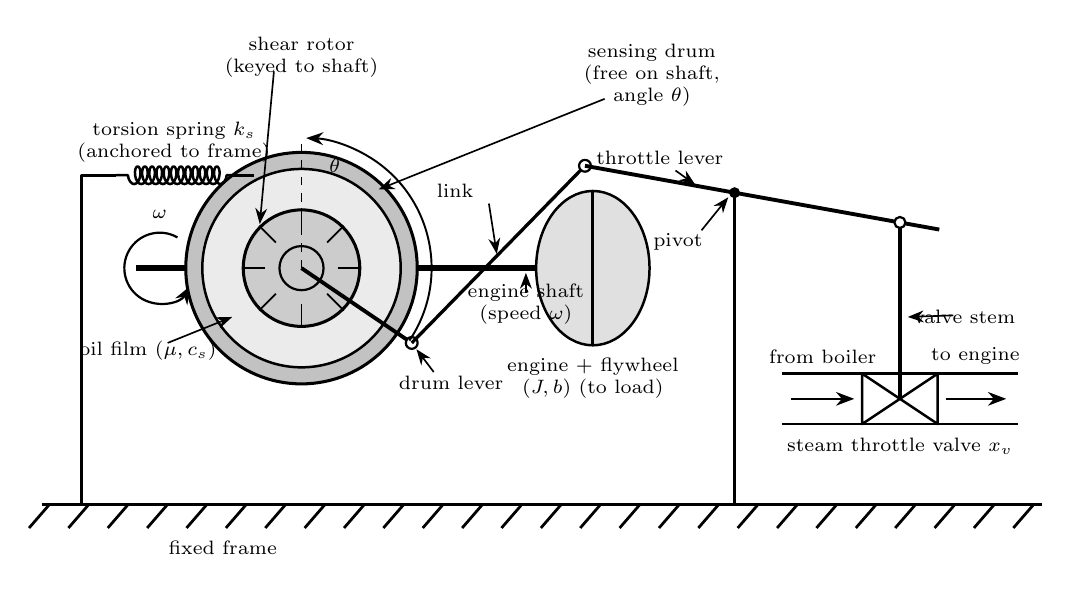
\begin{tikzpicture}[>=Stealth,font=\scriptsize,line join=round]
\def\gy{-3.0}
% ---------------- fixed frame -------------------------------------
\draw[line width=1pt] (-1.8,\gy) -- (10.9,\gy);
\foreach \x in {-1.7,-1.2,...,10.8}{\draw[line width=1pt] (\x,\gy)--(\x-0.26,\gy-0.30);}
\node[below,font=\scriptsize] at (0.5,\gy-0.34){fixed frame};

% ---------------- engine shaft, engine and flywheel ---------------
\draw[line width=2.3pt] (-0.60,0) -- (5.92,0);
\fill[black!12] (5.20,0) ellipse (0.72 and 0.98);
\draw[line width=0.9pt] (5.20,0) ellipse (0.72 and 0.98);
\draw[line width=1.1pt] (5.20,0.98) -- (5.20,-0.98);
\node[font=\scriptsize,align=center] at (4.35,-0.46){engine shaft\\(speed $\omega$)};
\draw[->,line width=0.6pt] (4.35,-0.32) -- (4.35,-0.06);
\node[font=\scriptsize,align=center,below] at (5.20,-1.02){engine $+$ flywheel\\ $(J,b)$ (to load)};
\draw[->,line width=0.8pt] (-0.075,0.390) arc [start angle=60,end angle=330,radius=0.45];
\node[font=\scriptsize] at (-0.30,0.68){$\omega$};

% ---------------- oil chamber: drum ring, film, rotor -------------
% Three separate parts, drawn in this order: the sensing drum (a ring, the
% chamber wall), the oil film (the annulus between drum bore and rotor), and
% the shear rotor (a solid disc keyed to the shaft).
\fill[black!24] (1.5,0) circle (1.47);   % sensing drum
\fill[black!8]  (1.5,0) circle (1.26);   % oil film
\fill[black!20] (1.5,0) circle (0.74);   % shear rotor
\draw[line width=1.1pt] (1.5,0) circle (1.47);
\draw[line width=0.9pt] (1.5,0) circle (1.26);
\draw[line width=1.1pt] (1.5,0) circle (0.74);
\draw[line width=0.8pt] (1.5,0) circle (0.28);
\foreach \a in {0,45,...,315}{\draw[line width=0.6pt] ($(1.5,0)+(\a:0.46)$) -- ($(1.5,0)+(\a:0.76)$);}

% one leader per part, each landing on that part --------------------
\node[font=\scriptsize,align=center] at (1.5,2.68){shear rotor\\(keyed to shaft)};
\draw[->,line width=0.6pt] (1.15,2.50) -- (0.97,0.56);
\node[font=\scriptsize,align=center] at (5.95,2.45){sensing drum\\ (free on shaft,\\ angle $\theta$)};
\draw[->,line width=0.6pt] (5.35,2.15) -- (2.48,1.00);
\node[font=\scriptsize,align=center] at (-0.45,-1.05){oil film ($\mu,c_s$)};
\draw[->,line width=0.6pt] (-0.20,-0.95) -- (0.62,-0.62);

% ---------------- torsion spring, on a drum lug, anchored to frame
\draw[line width=1.0pt] (0.90,1.18) -- (0.62,1.18);
\draw[decorate,decoration={coil,segment length=2.6pt,amplitude=3.2pt,pre length=2pt,post length=2pt},
      line width=0.9pt] (0.62,1.18) -- (-0.86,1.18);
\draw[line width=1.1pt] (-0.86,1.18) -- (-1.30,1.18) -- (-1.30,\gy);
\node[font=\scriptsize,align=center,above] at (-0.12,1.22){torsion spring $k_s$\\ (anchored to frame)};

% ---------------- drum lever -------------------------------------
\draw[line width=1.4pt] (1.5,0) -- (2.90,-0.95);
\fill[white] (2.90,-0.95) circle (0.075);
\draw[line width=0.8pt] (2.90,-0.95) circle (0.075);
\node[font=\scriptsize,align=center] at (3.40,-1.45){drum lever};
\draw[->,line width=0.6pt] (3.18,-1.32) -- (2.96,-1.03);

% ---------------- link to the throttle lever ---------------------
\draw[line width=1.2pt] (2.90,-0.95) -- (5.10,1.30);
\fill[white] (5.10,1.30) circle (0.075);
\draw[line width=0.8pt] (5.10,1.30) circle (0.075);
\node[font=\scriptsize] at (3.45,0.98){link};
\draw[->,line width=0.6pt] (3.88,0.82) -- (3.98,0.18);

% ---------------- throttle lever ---------------------------------
% The link attaches to the LEFT of the pivot and the valve stem to the RIGHT
% of it, so a rise in speed lowers the stem and CLOSES the valve.  This is the
% sense reversal; it is visible because the stem is on the far side of the pin.
\draw[line width=1.4pt] (5.10,1.30) -- (9.60,0.49);
\coordinate (Pv) at (7.00,0.958);
\draw[line width=1.1pt] (Pv) -- (7.00,\gy);
\fill[black] (Pv) circle (0.07);
\node[font=\scriptsize,align=center] at (6.05,1.40){throttle lever};
\draw[->,line width=0.6pt] (6.25,1.24) -- (6.50,1.06);
\node[font=\scriptsize,align=center] at (6.28,0.34){pivot};
\draw[->,line width=0.6pt] (6.58,0.48) -- (6.92,0.90);

% ---------------- valve stem + gate valve ------------------------
\draw[line width=1.2pt] (9.10,0.58) -- (9.10,-1.66);
\fill[white] (9.10,0.58) circle (0.07);
\draw[line width=0.8pt] (9.10,0.58) circle (0.07);
\node[font=\scriptsize,align=center] at (9.92,-0.62){valve stem};
\draw[->,line width=0.6pt] (9.78,-0.60) -- (9.20,-0.62);

% ---------------- steam pipe (horizontal) ------------------------
\draw[line width=1.0pt] (7.60,-1.34) -- (10.60,-1.34);
\draw[line width=1.0pt] (7.60,-1.98) -- (10.60,-1.98);
% gate valve symbol (bow-tie) at the stem
\draw[line width=0.9pt] (9.10,-1.66) -- (8.62,-1.34) -- (8.62,-1.98) -- cycle;
\draw[line width=0.9pt] (9.10,-1.66) -- (9.58,-1.34) -- (9.58,-1.98) -- cycle;
\node[font=\scriptsize,align=center,below] at (9.10,-2.04){steam throttle valve $x_v$};
\draw[->,line width=0.8pt] (7.72,-1.66) -- (8.52,-1.66);
\node[font=\scriptsize,above] at (8.12,-1.34){from boiler};
\draw[->,line width=0.8pt] (9.68,-1.66) -- (10.45,-1.66);
\node[font=\scriptsize,above] at (10.06,-1.34){to engine};

% ---------------- drum rotation indicator ------------------------
\draw[dashed,line width=0.6pt] (1.5,0) -- (1.5,1.65);
\draw[->,line width=0.7pt] (2.87,-0.92) arc [start angle=-34,end angle=88,radius=1.65];
\node[font=\scriptsize] at (1.92,1.30){$\theta$};
\end{tikzpicture}}
\caption{Engineering schematic of the viscous-drag governor. A shear rotor keyed to
the engine shaft shears the oil film in the sealed chamber; the shear torque is
balanced by a torsion spring anchored to the frame, so the sensing drum (free on the
shaft) settles at a deflection $\theta$ proportional to engine speed. The drum lever
and link transmit $\theta$ to the throttle lever, and the link and the valve stem lie
on \emph{opposite} sides of the pivot, so the stem descends and closes the steam
valve as speed rises ($K_l=\mathrm{d}x_v/\mathrm{d}\theta$). Counted from the
drawing, the linkage has five plain turning pairs: the drum bearing, the two link
pins, the throttle-lever pivot and the valve-stem joint.}
\label{fig:schematic}
\end{figure*}

%--------------------------------------------------------------------
\begin{figure}[t]
\centering
\resizebox{\columnwidth}{!}{%
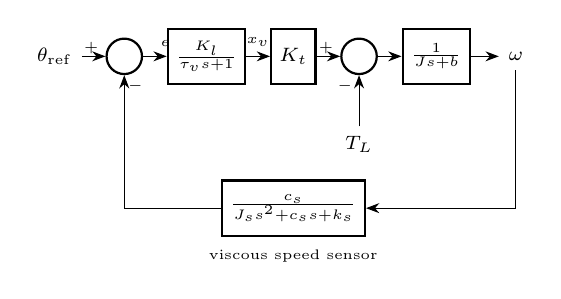
\begin{tikzpicture}[>=Stealth,font=\scriptsize,
   blk/.style={draw,line width=0.8pt,minimum height=7mm,inner xsep=3pt,align=center},
   sm/.style={draw,circle,line width=0.8pt,inner sep=0pt,minimum size=4.5mm}]
\node (ref) {$\theta_{\mathrm{ref}}$};
\node[sm,right=3mm of ref] (s1) {};
\node[blk,right=3mm of s1] (gv) {$\frac{K_l}{\tau_vs+1}$};
\node[blk,right=3mm of gv] (kt) {$K_t$};
\node[sm,right=3mm of kt] (s2) {};
\node[blk,right=3mm of s2] (gp) {$\frac{1}{Js+b}$};
\node[right=3.5mm of gp] (om) {$\omega$};

\draw[->] (ref) -- (s1);
\draw[->] (s1) -- (gv);
\node[above,font=\tiny] at ($(s1)!0.5!(gv)$) {$e$};
\draw[->] (gv) -- node[above,font=\tiny]{$x_v$} (kt);
\draw[->] (kt) -- (s2);
\draw[->] (s2) -- (gp);
\draw[->] (gp) -- (om);

% The load torque must enter AFTER the throttle gain K_t, so that Eq. (15)
% reads -1/(Js+b) and the disturbance does not pick up a spurious factor K_t.
\node[below=6.5mm of s2,font=\scriptsize] (tl) {$T_L$};
\draw[->] (tl) -- (s2);
\node[font=\tiny] at ([xshift=-1.8mm,yshift=1.1mm]s2.west)  {$+$};
\node[font=\tiny] at ([xshift=-1.8mm,yshift=-1.4mm]s2.south){$-$};
\node[font=\tiny] at ([xshift=-1.8mm,yshift=1.1mm]s1.west)  {$+$};

% The viscous sensor lies in the FEEDBACK path: a drum driven by the oil film
% measures shaft speed omega, never the error e = theta_ref - theta.
\node[blk,below=12mm of kt] (hh) {$\frac{c_s}{J_ss^{2}+c_ss+k_s}$};
\node[below=0.4mm of hh,font=\tiny] {viscous speed sensor};
\draw[->] (om) |- (hh.east);
\draw[->] (hh.west) -| (s1.south);
\node[font=\tiny] at ([xshift=1.4mm,yshift=-1.4mm]s1.south) {$-$};
\end{tikzpicture}}
\caption{Closed-loop block diagram. The viscous sensor sits in the \emph{feedback}
path, because an oil-film drum measures shaft speed $\omega$ and cannot sense the
error directly; it produces the drum angle $\theta$, compared with the setpoint
$\theta_{\mathrm{ref}}$ set by the calibrated stop on the valve lever. The load
torque $T_L$ enters \emph{after} the throttle gain $K_t$, at the shaft, as
Eq.~\eqref{eq:Gd} requires. Grouping the sensor with the valve gives the equivalent
controller $G_c(s)$ of Eq.~\eqref{eq:Gc}, with
$G_p(s)=K_t/[(Js+b)(\tau_vs+1)]$.}
\label{fig:block}
\end{figure}

%=====================================================================
\section{Mathematical Modeling}\label{sec:model}
%=====================================================================
\subsection{Nonlinear Governing Equations}
Let $\omega$ be the shaft speed. The driven machinery of a mill is a mixture of
constant-torque machines (looms, hammers) and speed-dependent machines (fans,
pumps, and the viscous drag of belts and journals), so the load torque is written as
the nonlinear function
\begin{equation}
T_L(\omega)=T_a+c_1\omega+c_2\omega^{2},
\label{eq:TL}
\end{equation}
in which the constant $T_a$ represents looms and hammers, the linear term
$c_1\omega$ journal and belt friction, and the quadratic term $c_2\omega^{2}$ fans
and pumps; $T_e(t)$ is the switched torque of a machine engaged or
disengaged---precisely the disturbance the governor must reject. With a
constant-cutoff steam
admission the indicated torque is proportional to throttle opening, and the shaft
equation is
\begin{equation}
J\dot\omega=K_t\,x_v-T_L(\omega).
\label{eq:shaft}
\end{equation}
The sensing drum obeys angular momentum balance with the film torque of
Eq.~\eqref{eq:newton} and the spring torque,
\begin{equation}
J_s\ddot\theta+c_s\dot\theta+k_s\theta=c_s\,\omega,
\label{eq:drum}
\end{equation}
and the throttle valve is a first-order lag driven by the linkage,
\begin{equation}
\tau_v\dot x_v+x_v=K_l\bigl(\theta_{\mathrm{ref}}-\theta\bigr).
\label{eq:valve}
\end{equation}
Equations~\eqref{eq:shaft}--\eqref{eq:valve} are the nonlinear model. The
nonlinearity resides in $T_L(\omega)$ (quadratic drag of the driven machinery) and
would also appear in a nonlinear valve flow--lift law.

\subsection{Linearisation}
Choose the nominal operating point $\omega_0=1$, $T_{L0}=T_L(\omega_0)=1$,
$x_{v0}=1$ and $\theta_0=c_s\omega_0/k_s$. Writing $\omega=\omega_0+\delta\omega$
and similarly for the other variables, and expanding Eq.~\eqref{eq:TL} to first
order, the load torque perturbation is
$\delta T_L=b\,\delta\omega+\delta T_{L,e}$, where
\begin{equation}
b\;\triangleq\;\left.\frac{\mathrm dT_L}{\mathrm d\omega}\right|_{\omega_0}
=c_1+2c_2\omega_0
\label{eq:bdef}
\end{equation}
is the \emph{effective viscous damping} and $\delta T_{L,e}$ is the external step
disturbance. For the design used here $T_a=0.25$, $c_1=0.5$ and $c_2=0.25$, so that
$T_L(\omega_0)=1$ and $b=c_1+2c_2\omega_0=1$: this is the physical origin of $b$,
which lumps journal friction together with the velocity-dependent drag of the mill.
Equation~\eqref{eq:shaft} at the nominal point then requires
$K_tx_{v0}=T_{L0}=1$, so with $x_{v0}=1$ the throttle gain is $K_t=1$---the damping
torque is \emph{inside} $T_L$ and must not be counted a second time in the
steady-state balance. The linearised system is therefore
\begin{align}
J\,\delta\dot\omega &= K_t\,\delta x_v-b\,\delta\omega-\delta T_{L,e},\label{eq:lin1}\\
J_s\,\delta\ddot\theta+c_s\,\delta\dot\theta+k_s\,\delta\theta&=c_s\,\delta\omega,\label{eq:lin2}\\
\tau_v\,\delta\dot x_v+\delta x_v&=-K_l\,\delta\theta.\label{eq:lin3}
\end{align}
Note that Eq.~\eqref{eq:lin2} is already linear: the VDG needs no linearisation of
its own sensing element.

\subsection{Plant and Controller Transfer Functions}
Taking Laplace transforms of Eqs.~\eqref{eq:lin1}--\eqref{eq:lin3}, the plant is
\begin{equation}
G_p(s)=\frac{\delta\omega}{\delta x_v}
=\frac{K_t}{(Js+b)(\tau_vs+1)}
=\frac{1}{(10s+1)(0.1s+1)},
\label{eq:Gp}
\end{equation}
and the controller, taken from the speed error
$e=\omega_{\mathrm{ref}}-\omega$ to the commanded throttle, is
\begin{equation}
\begin{aligned}
G_c(s)&=\frac{\delta x_v}{e}=\frac{16}{0.02\,s^{2}+0.2\,s+1},\\
&=\frac{K_l\,(c_s/k_s)}{(J_s/k_s)\,s^{2}+(c_s/k_s)\,s+1}.
\end{aligned}
\label{eq:Gc}
\end{equation}
With the parameters of Table~\ref{tab:params} the DC loop gain is
$G_0=G_c(0)G_p(0)=K_tK_lc_s/(k_sb)=16$.

\subsection{Closed-Loop Transfer Functions}
The loop transfer function is
\begin{equation}
\begin{split}
L(s)&=G_c(s)G_p(s)\\
&=\frac{16}{0.02s^{4}+0.402s^{3}+3.04s^{2}+10.3s+1},
\end{split}
\label{eq:L}
\end{equation}
so the closed-loop transfer function from the speed setpoint to the speed is
\begin{equation}
\begin{split}
G_{CL}(s)&=\frac{\omega(s)}{\omega_{\mathrm{ref}}(s)}=\frac{L(s)}{1+L(s)}\\
&=\frac{16}{0.02s^{4}+0.402s^{3}+3.04s^{2}+10.3s+17}.
\end{split}
\label{eq:GCL}
\end{equation}
Because the load torque is applied directly at the shaft, the disturbance transfer
function is different and is the quantity that governs the \emph{regulation}
problem:
\begin{equation}
\begin{split}
\frac{\omega(s)}{T_L(s)}&=\frac{-1/(Js+b)}{1+G_cG_p}\\
&=\frac{-(0.1s+1)\,(0.02s^{2}+0.2s+1)}
{0.02s^{4}+0.402s^{3}+3.04s^{2}+10.3s+17}.
\end{split}
\label{eq:Gd}
\end{equation}
The DC gain of Eq.~\eqref{eq:Gd} is the speed droop of a type-0 loop~\cite{dorf},
\begin{equation}
\text{droop}=\left|\frac{\omega(\infty)}{T_L(\infty)}\right|
=\frac{1}{b\,(1+G_0)}=\frac{1}{17}=5.88\%,
\label{eq:droop}
\end{equation}
i.e.\ a full (100\%) change of load torque produces a $5.88\%$ permanent speed
change. For the $\pm30\%$ steps specified in the brief this is only $\pm1.76\%$.

\subsection{Reset (Integral) Variant}
The residual droop of Eq.~\eqref{eq:droop} can be removed by a standard mechanical
\emph{reset}: a viscous dashpot is inserted between the linkage and the spring
anchor so that a persistent deflection slowly re-trims the spring seat until the
error vanishes. This multiplies Eq.~\eqref{eq:Gc} by the factor $(T_is+1)/(T_is)$ with
$T_i=4$~s, which contains an integrator and therefore forces zero steady-state
error. The resulting fifth-order characteristic polynomial, from $1+G_cG_p=0$, is
$0.08s^{5}+1.608s^{4}+12.16s^{3}+41.2s^{2}+68s+16=0$.

%=====================================================================
\section{Control and Stability Analysis}
%=====================================================================
\subsection{Routh--Hurwitz Analysis}
Closed-loop stability is the classical problem first posed by
Maxwell~\cite{maxwell}. Substituting Eqs.~\eqref{eq:Gc} and~\eqref{eq:Gp} into
$1+G_cG_p=0$ gives the closed-loop characteristic polynomial
\begin{equation}
0.02s^{4}+0.402s^{3}+3.04s^{2}+10.3s+17=0 .
\label{eq:char}
\end{equation}
The Routh first column is $(0.02,\,0.402,\,2.528,\,7.596,\,17)$, all strictly
positive, so by the Routh--Hurwitz criterion~\cite{nise} the closed loop is
asymptotically stable; the binding $s^{1}$ element,
$c_1=(b_1a_1-a_3a_0)/b_1=7.60>0$, confirms it. The same array gives the gain at
which stability is lost: $G_0^{\mathrm{crit}}=63.8$, or $3.99$ times the design
value of $16$, in agreement with the $12.0$~dB gain margin found below.

\subsection{Closed-Loop Poles}
Solving Eq.~\eqref{eq:char} gives
\begin{equation}
s_{1,2}=-2.432\pm j2.685,\quad s_{3,4}=-7.618\pm j2.595\ \ [\mathrm{rad/s}].
\label{eq:poles}
\end{equation}
The pair $s_{1,2}$ lies closest to the imaginary axis and therefore dominates the
response, with $\omega_n=3.62$~rad/s and $\zeta=0.671$. This damping ratio
corresponds to an equivalent second-order overshoot of $5.8\%$; the observed $4.6\%$
(Sec.~\ref{sec:sim}) is slightly smaller because the distant pair $s_{3,4}$
(\mbox{$\zeta\approx0.95$}) adds a small in-phase component. The dominant real part
($-2.43$) sets the response speed: a loop time constant of $0.41$~s against the
plant's $J/b=10$~s, i.e.\ feedback makes the governed engine about $20\times$ faster
while cutting its load sensitivity by a factor of $17$.

\subsection{Frequency-Response Margins}
The loop transfer function~\eqref{eq:L} has its gain crossover at
$\omega_c=1.575$~rad/s, giving
\begin{equation}
\mathrm{PM}=66.3\dg,\qquad \mathrm{GM}=12.0\ \mathrm{dB}\ \text{at}\ 5.06\ \mathrm{rad/s}.
\label{eq:margins}
\end{equation}
The margin remains sufficient because the crossover lies well below both the
sensing-drum natural frequency ($\omega_{n,s}=\sqrt{k_s/J_s}=7.07$ rad/s) and the
valve corner ($1/\tau_v=10$ rad/s), so little phase lag enters inside the loop
bandwidth. This is the central design rule of the VDG: \emph{the drum must be stiff
and light relative to the loop bandwidth}.

\subsection{The Reset Variant}
For the reset design of Sec.~\ref{sec:model} the closed-loop poles are
\begin{equation}
-7.497\pm j2.537,\quad -2.413\pm j2.374,\quad -0.279\ \ [\mathrm{rad/s}],
\label{eq:polesPI}
\end{equation}
with PM $=57.1\dg$ and GM $=11.6$~dB; the Routh first column
($0.08,1.608,10.11,30.51,61.90,16$) is entirely positive, so the reset loop is also
stable. The real pole at $-0.279$ is dominant and reflects the reset time constant
$T_i$, the price paid for zero droop: integral action removes the offset but costs
$9\dg$ of phase margin and slows the final settling.

%=====================================================================
\section{Simulation and Results}\label{sec:sim}
%=====================================================================
\subsection{Method and Parameters}
The model was implemented in MATLAB R2025b (Octave-compatible scripts; repository
link in the footnote) and integrated with a classical fourth-order Runge--Kutta
scheme, fixed step $2$~ms over $80$~s, so no toolbox function is required. Step
disturbances from $T_L=1$ to $1.3$ and to $0.7$ were applied; the open-loop case is
the same plant with the throttle held at $x_{v0}=1$.

Table~\ref{tab:params} lists the parameters with their dimensional anchors. A
nominal speed of $60$~rpm and power of $20$~kW give $3183$~N$\cdot$m of torque, so
$J=10$ represents a $2$~t flywheel of $1.6$~m radius of gyration---typical of a mill
engine---and $J_s$ a $1.3$~kg drum shell of $0.40$~m radius, consistent with
Fig.~\ref{fig:schematic}. The linkage gain $K_l=80$ is realised by a $0.40$~m drum
radius feeding a $20$:$1$ compound lever.

\subsection{Open-Loop Versus Closed-Loop Response}
Fig.~\ref{fig:response} compares the two cases. Without a governor a $+30\%$ load
step drives the speed from $1$ to $0.700$, a \emph{$30\%$} steady-state error
reached with the plant's slow $10$~s time constant; the $-30\%$ step is exactly
symmetric, with the speed rising to $1.300$. This near-proportional load--speed
relationship is the historical failure mode of the brief and follows directly from
the normalisation $b\,\omega_0=T_{L0}$.

With the VDG closed the same $+30\%$ step gives a peak deviation of only $1.85\%$
($\omega=0.9815$) and a steady-state error of $1.76\%$ ($\omega_\infty=0.9824$),
reached after $1.58$~s ($2\%$ of the final change); the $-30\%$ step is symmetric
($\omega_\infty=1.0176$). The response is monotonic to within the band, with a
$4.6\%$ overshoot relative to its final value, consistent with $\zeta=0.671$, and the
dominant-pair angle of $48\dg$ gives $\zeta=\cos48\dg=0.67$ as computed
analytically. The throttle moves $0.282$ normalised units ($28\%$ of the nominal
opening, within the half-open starting position of Sec.~\ref{sec:intro}), driven by
the $1.3\dg$ drum rotation predicted by $\delta\theta=(c_s/k_s)\,\delta\omega$.

\subsection{Effect of the Reset}
Table~\ref{tab:results} contrasts the proportional design with the reset (PI) design
and collects all metrics. The reset drives the steady-state
error to zero and the peak deviation slightly \emph{down}, from $1.85\%$ to
$1.77\%$: adding $1/(T_is)$ raises the loop gain at every frequency below
crossover, so the reset response is bounded in magnitude by the proportional one.
The price is a longer tail: the reset enters the $\pm0.5\%$ band at $5.5$~s, against
$1.58$~s for the proportional design to enter its $\pm2\%$ band. Which
design is preferred depends on the duty: the
proportional version is the simpler and slightly better damped mechanism and is the
one recommended for the mill drive, where a $1.76\%$ speed change under a $30\%$
load step is already an order of magnitude better than anything a
1780s engine could otherwise achieve; the reset version is recommended where
several engines must run in parallel and be synchronised, since integral action
removes the standing droop that would otherwise accumulate into a phase error.

\begin{table}[t]
\caption{Model parameters. Normalised values are those of Eqs.~(2)--(17); physical
values follow from the scales $\tau_0=1$~s, $\omega_0=6.283$~rad/s (60~rpm),
$T_0=3183$~N$\cdot$m (20~kW) and $\theta_0=\omega_0\tau_0$.}
\label{tab:params}
\centering
\footnotesize
\begin{tabular}{@{}lll>{\raggedright\arraybackslash}p{3.2cm}@{}}
\toprule
Symbol & Norm. & Physical & Basis \\
\midrule
$J$      & $10$     & $5.1\times10^{3}$ kg$\cdot$m$^2$ & flywheel $+$ engine; spin-down time $J/b=10$ s \\
$b$      & $1$      & $507$ N$\cdot$m$\cdot$s/rad & slope of $T_L$ at $\omega_0$; $b\omega_0=T_{L0}$ \\
$K_t$    & $1$      & --- & nominal balance $K_tx_{v0}=T_{L0}=1$ \\
$\tau_v$ & $0.1$ s  & $0.1$ s & valve lag; $\approx1.6$~Hz bandwidth of the stem $+$ lever \\
$J_s$    & $4\!\times\!10^{-4}$ & $0.20$ kg$\cdot$m$^2$ & sensor time constant $J_s/k_s=0.02$ s$^{2}$ \\
$c_s$    & $4\!\times\!10^{-3}$ & $2.0$ N$\cdot$m$\cdot$s/rad & film transmits $12.7$ N$\cdot$m ($80$ W) at $\omega_0$ \\
$k_s$    & $0.02$   & $10.1$ N$\cdot$m/rad & $\theta_{ss}=72\dg$ full scale, $1.3\dg$ per load step \\
$K_l$    & $80$     & --- & linkage gain; sets $G_0=16$ \\
$T_i$    & $4$ s    & $4$ s & reset: shortest tail that still keeps PM $>55\dg$ \\
\bottomrule
\end{tabular}
\vspace{2pt}
{\scriptsize\raggedright $J$, $b$, $K_t$, $\tau_v$ follow from the stated engine and the
nominal torque balance; the sensor and linkage entries were \emph{fitted} to meet the
design targets, their absolute scale then being set by the drum size and the
film-dissipation limit (appendix).
\par}
\end{table}

\begin{table}[t]
\caption{Transient-response metrics for $\pm30\%$ step load disturbances
(normalised variables, $\omega_0=1$, $T_{L0}=1$)}
\label{tab:results}
\centering
\footnotesize
\setlength{\tabcolsep}{3.2pt}
\begin{tabular}{@{}lccccc@{}}
\toprule
Case & $\omega_\infty$ & err.\ & peak & $t_s$ & $x_{v\infty}$ \\
     &                & $[\%]$ & $[\%]$ & $[\mathrm s]$ & \\
\midrule
\multicolumn{6}{@{}l}{\emph{$+30\%$ load step ($T_L:1\to1.3$)}}\\
Open loop      & $0.700$ & $30.0$ & $30.0$ & $38.96$ & $1.000$ \\
VDG ($P$)      & $0.982$ & $1.76$  & $1.85$  & $1.58$  & $1.282$ \\
VDG ($P$+reset)& $1.000$ & $0.00$  & $1.77$  & $5.5$   & $1.300$ \\
\midrule
\multicolumn{6}{@{}l}{\emph{$-30\%$ load step ($T_L:1\to0.7$)}}\\
Open loop      & $1.300$ & $30.0$ & $30.0$ & $38.96$ & $1.000$ \\
VDG ($P$)      & $1.018$ & $1.76$  & $1.85$  & $1.58$  & $0.718$ \\
VDG ($P$+reset)& $1.000$ & $0.00$  & $1.77$  & $5.5$   & $0.700$ \\
\bottomrule
\end{tabular}
\vspace{2pt}
{\scriptsize\raggedright $t_s$: time to enter the $\pm2\%$ band about $\omega_\infty$;
for the reset rows, whose final error is zero, the $\pm0.5\%$ band. For the open loop
``peak'' is the final error (monotone response), for the governor the transient
excursion. The reset peak is below the $P$ peak because integral action only raises
the loop gain.
\par}
\end{table}

%--------------------------------------------------------------------
\begin{figure*}[t]
\centering
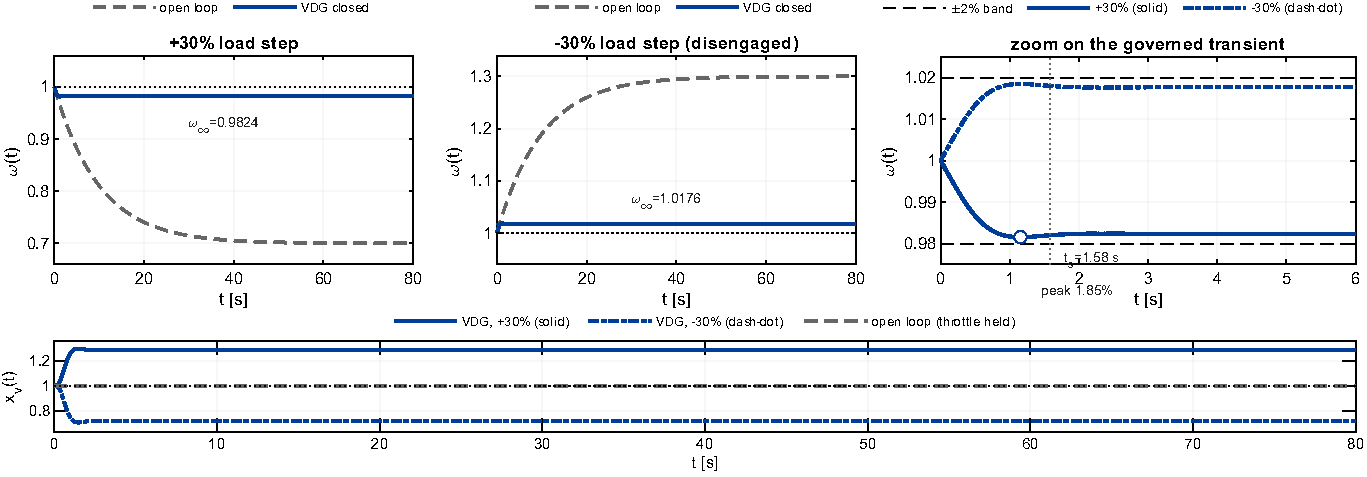
\includegraphics[width=0.74\textwidth]{fig_open_closed.pdf}
\caption{Open-loop versus closed-loop response to the prescribed load steps. Top
row: engine speed $\omega(t)$ for a $+30\%$ step, for a $-30\%$ step (machine
disengaged), and a zoom on the governed transient that makes the $1.85\%$ peak and
the $1.58$~s settling time visible. Bottom: throttle position $x_v(t)$. The ungoverned
engine changes speed by $30\%$ and takes $\approx39$~s to settle. Colour is fixed
across every panel: grey dashed $=$ open loop, blue $=$ governed; the sign of the step
is given by the title or the line style.}
\label{fig:response}
\end{figure*}

%=====================================================================
\section{Conclusions}\label{sec:conclusions}
%=====================================================================
\subsection{Summary}
A new speed governor has been invented in which the centrifugal flyweights of every
historical governor are replaced by a viscous-shear sensing element: a rotor shears
an oil film that deflects a spring-restrained sensing drum, giving a speed signal
\emph{linear} in $\omega$ rather than quadratic. A first-principles nonlinear model
was derived and linearised about the normalised operating point, yielding $G_p(s)$,
$G_c(s)$, $G_{CL}(s)$ and a fourth-order characteristic polynomial. Routh--Hurwitz
analysis proves asymptotic stability (first column $0.02,0.402,2.528,7.596,17$) with
a phase margin of $66.3\dg$, a gain margin of $12.0$~dB and a dominant pair at
$\omega_n=3.62$~rad/s, $\zeta=0.671$. Under the prescribed $\pm30\%$ load steps the
governor cuts the speed error from $30\%$ to $1.76\%$, with a $1.85\%$ peak deviation
and a $1.58$~s settling time, while a viscous reset drives the error to zero.

\subsection{Advantages}
\begin{enumerate}
\item The sensing law is linear, so the loop gain is independent of working speed
and the governor behaves almost identically at low and high speed, which a flyball
governor can only approximate.
\item Fewer moving parts: the sensor adds one plain bearing and a three-bar
linkage---five turning pairs (Fig.~\ref{fig:schematic})---whereas a flyball assembly
needs flyweights, a sliding sleeve, links and their pivots, the rubbing sleeve being
the part that dominates its wear.
\item The oil film is self-damping, so the sensor adds useful loop damping rather
than the lightly damped resonance of a spring--flyweight system.
\item Every component---cast-iron drum, brass chamber, steel torsion spring, leather
seals, vegetable oil---was available to an eighteenth-century instrument maker.
\end{enumerate}

\subsection{Limitations and Failure Modes}
\begin{enumerate}
\item \textbf{Viscosity drift---the dominant limitation.} The gain
$c_s=\mu Ar^{2}/h$ is proportional to $\mu$, and a rise in oil temperature from
$15\dg$C to $50\dg$C lowers a vegetable oil's $\mu$ about threefold. With the setpoint
fixed by the stop $\theta_{\mathrm{ref}}$, the static balance gives
$\omega_\infty=K_l\theta_{\mathrm{ref}}/(1+K_lc_s/k_s)$, so the speed varies as
$1/c_s$: here $\omega_\infty=17/(1+16\,c_s/c_{s,0})$, so a threefold drop in $c_s$
raises the speed to $2.7\,\omega_0$ while the loop gain falls from $16$ to $5.3$ and
the droop rises from $5.9\%$ to $15\%$. This is runaway overspeed,
not graceful degradation, so active compensation is not optional. A bimetallic strip
closing the film gap as the oil warms helps ($c_s\propto1/h$), but holding
$\omega_\infty$ within $1\%$ demands $\mu/h$ to about $1\%$---best met by a
temperature-stable oil in a thermally inert chamber.
\item \textbf{Leakage and contamination.} Oil loss through the shaft seal lowers the
transmitted torque and emulsion with steam condensate raises $\mu$; both change the
calibration rather than causing failure, so the governor degrades gracefully.
\item \textbf{Friction and stiction.} The film transmits only $12.7$ N$\cdot$m at
rated speed, so bearing friction is a fixed fraction of the signal. A friction
torque $T_f$ makes the drum
stick until $c_s\,\delta\omega=T_f$, so the dead band is
$\delta\omega/\omega_0=T_f/(c_s\omega_0)=T_f/12.7$ N$\cdot$m. For a bronze journal of
radius $r=25$~mm, $\mu_f=0.1$ and a normal load $N=10$~N (the drum's weight share),
$T_f=\mu_fNr=0.025$ N$\cdot$m and the dead band is $0.2\%$ of rated speed---half the
$\pm0.5\%$ band. Hardened, oil-lubricated pivots or a jewel-and-pin arrangement are
therefore required.
\item \textbf{Backlash and resolution---the least severe mode.} A $30\%$ load step
moves the drum through $1.3\dg$, so $0.05$~mm of slack in the lever pins amounts to
only $0.007\dg$ at the drum; the large working travel makes backlash far less
critical here than in the small-arc linkage of a flyball governor.
\item \textbf{Spring creep and aeration.} A steel torsion spring relaxes slowly
under load, drifting the setpoint, and high shear entrains air that slowly reduces
the transmitted torque. Periodic recalibration (or a leaf spring stressed well below
its elastic limit) and a generous, baffled chamber address both.
\end{enumerate}

\subsection{Proposed Improvements}
In order of value: (i) add the viscous reset dashpot of Sec.~\ref{sec:model} to
eliminate droop; (ii) make the film thickness $h$ adjustable so that $c_s$ can be
re-trimmed in service; (iii) add a parallel air dashpot across the lever to raise
loop damping at constant DC gain; (iv) harden and anti-backlash the lever; (v) add a
temperature-compensating element against the daily swing of a mill.

%=====================================================================
\begin{thebibliography}{9}
\bibitem{maxwell} J. C. Maxwell, ``On governors,'' \emph{Proceedings of the Royal
Society of London}, vol.~16, pp.~270--283, 1868.
\bibitem{bennett} S. Bennett, \emph{A History of Control Engineering 1800--1930}.
Stevenage, U.K.: Peregrinus, 1979.
\bibitem{dickinson} H. W. Dickinson and J. Rhys Jenkins, \emph{James Watt and the
Steam Engine}. Oxford, U.K.: Clarendon Press, 1927.
\bibitem{nise} N. S. Nise, \emph{Control Systems Engineering}, 8th ed. Hoboken, NJ:
Wiley, 2019.
\bibitem{dorf} R. C. Dorf and R. H. Bishop, \emph{Modern Control Systems}, 13th ed.
Pearson, 2017.
\bibitem{munson} B. R. Munson, D. F. Young and T. H. Okiishi, \emph{Fundamentals of
Fluid Mechanics}, 5th ed. Wiley, 2006.
\end{thebibliography}

\clearpage
\section*{Appendix: Use of Artificial Intelligence}
\markboth{Appendix: Use of Artificial Intelligence}{Appendix: Use of Artificial Intelligence}

\textbf{Tools used.} (a)~\emph{AI assistant}: Buffy (DeepSeek V4.1 Flash, inside
the Freebuff client), used as a pair-programming and drafting assistant, including
the repair of LaTeX layout faults (over-long display equations, a block diagram
that overflowed its column, badly stretched table cells). (b)
\emph{Typesetting}: pdfLaTeX (MiKTeX~25.12) with the \texttt{IEEEtran} conference
class, \texttt{amsmath}, \texttt{booktabs} and TikZ/PGF for the schematic and the
block diagram. (c)~\emph{Numerics}: MATLAB~R2025b for the linear algebra, root
finding, Runge--Kutta integration, frequency response and every figure; the scripts
use base MATLAB/Octave functions only, so they carry no toolbox dependency. (d)
Python~3 with NumPy/SciPy, used as a scratchpad for the parameter search. (e)~Git
and GitHub for version control. (f)~Two further AI assistants, Claude and Gemini,
used only as \emph{critics} of a complete draft (see below). No
computer-algebra package was needed: the linearisation was carried out by hand and
verified numerically. The governing equations, the choice of every parameter and
the reading of every result were the author's own; the assistant was used to draft
text, to write and debug code to the author's specification, and to check algebra.

\textbf{Prompts used and how each tool was used.} Prompts are quoted verbatim.
(1)~``Derive the governing equations of a viscous drag-cup governor: a rotor on the
engine shaft shearing an oil film that drags a spring-restrained sensing drum, with
the drum linked to a steam throttle.'' (2)~``Linearise these equations about
$\omega_0=1$, $T_{L0}=1$ and give $G_p(s)$, $G_c(s)$ and the closed-loop
characteristic polynomial.'' (3)~``Search the parameter space for a sensor
stiffness, film coefficient and lever gain that give a phase margin above $60\dg$
with a steady-state speed error below $2\%$ for a $30\%$ load step.'' (4)~``Write
Octave-compatible MATLAB that integrates the loop with a fixed-step RK4 and produces
the required transient plots.'' (5)~``Draft an IEEE-format section on why a
viscous-shear sensor is fundamentally different from a centrifugal flyweight
governor.'' In each case the author stated the physical requirement, the tool
returned a draft, and the author accepted, corrected or rejected it before it
entered the paper.

\textbf{Outputs accepted, modified and rejected.} \emph{Accepted after
verification:} the three-block loop structure (sensor$+$lever, valve, engine), the
RK4 integrator and the TikZ drawings. \emph{Rejected:} the assistant's first
parameter set, which placed the sensing-drum resonance below the loop crossover and
gave a phase margin of only $13\dg$ with a $76\%$ overshoot; the author rejected it
and raised the drum stiffness and the lever gain until the crossover fell below both
the drum and the valve corners (the design rule at the end of Sec.~IV-C).
\emph{Corrected by hand:} a sign error in the disturbance transfer function and an
error in the state-space realisation of the valve lag; both were found by checking
the computed steady-state error against the closed-form droop $1/(1+G_0)=5.88\%$.

\textbf{Parameters: what was fitted, and what was derived.} The quantities that set
the loop dynamics---$K_l$, $c_s/k_s$ and $J_s/k_s$---were \emph{fitted} by a
numerical search that swept them until the loop met the stated targets (phase margin
above $60\dg$, steady-state error below $2\%$ for a $30\%$ load step under a fixed
structure). The assistant ran that search. The absolute physical values were then
fixed separately by dimensional reasoning from the scales $\omega_0$, $T_0$ and
$\tau_0$ (Table~\ref{tab:params}), and $K_t$ was corrected to satisfy the nominal
torque balance. The failure modes of Sec.~VI-C were written by the author from
workshop reasoning about oil, brass and lever joints. Every number quoted in the
paper is regenerated by \texttt{vdg\_main.m} and none of it was accepted on trust.

\textbf{External review, and what it changed.} A complete draft was also submitted
for criticism to two further AI assistants, Claude and Gemini. Their comments led
directly to several of the corrections in this revision: the $K_t$ torque-balance
error, the mis-placed $T_L$ junction and the sensor's place in the feedback path of
Fig.~\ref{fig:block}, the $\theta_{ss}$ normalisation, the film's dissipation (and
the rescaling of the sensor from $637$~N$\cdot$m and $4$~kW to $12.7$~N$\cdot$m and
$80$~W), the quantified severity of viscosity drift, the author of~\cite{dickinson},
and removal of the pressurised-leak-path mitigation, which was physically empty for a
Couette film. No text was copied from those tools; each correction was checked
against the model and against the scripts before it was accepted.

\textbf{Figures, and what the review changed.} The same review, made on the rendered
PDF rather than on the source, found that the first version of
Fig.~\ref{fig:response} had been exported in the editor's dark theme (a near-black
axes background with pale grey labels, unreadable in print), that its legend boxes
covered the curves they labelled, that the governed colour changed from panel to
panel, and that the $1.85\%$ peak and the $1.58$~s settling time were invisible on an
$80$~s axis. All four were corrected: every figure is now exported light-on-white
with one colour and line style per case across all panels, legends are placed outside
the axes, the in-figure toolbar is suppressed, and an explicit zoom panel marks the
peak and the settling time. The proportional-versus-reset figure was dropped to hold
the six-page limit; its content is reported numerically in Table~\ref{tab:results}.

%=====================================================================
\end{document}
